\documentclass[11pt,a4paper]{article}

\usepackage[margin=2.5cm]{geometry}
\usepackage[T1]{fontenc}
\usepackage{lmodern}
\usepackage{graphicx}
\usepackage{float}
\usepackage[font=small,labelfont=bf]{caption}
\usepackage{booktabs}
\usepackage{array}
\usepackage[dvipsnames]{xcolor}
\usepackage{tikz}
\usetikzlibrary{positioning,arrows.meta,calc}
\usepackage{listings}
\usepackage[hidelinks]{hyperref}
\usepackage{soul}

\lstset{
  basicstyle=\ttfamily\small,
  breaklines=true,
  frame=single,
  columns=fullflexible,
  keepspaces=true
}

% \shot{filename.png}{caption}{label}
% Screenshots live in the Screenshots/ folder. A missing file shows a red box instead of breaking the build.
\newcommand{\shot}[3]{%
  \begin{figure}[H]
    \centering
    \IfFileExists{Screenshots/#1}%
      {\includegraphics[width=0.92\textwidth]{Screenshots/#1}}%
      {\fbox{\parbox{0.85\textwidth}{\centering\textcolor{red}{Missing screenshot:\\ \detokenize{#1}}}}}
    \caption{#2}\label{#3}
  \end{figure}}

\usepackage{titlesec}
\newcommand{\sectionbreak}{\clearpage}

\usepackage{tocloft}
\setlength{\cftbeforesecskip}{4pt}
\setlength{\cftbeforesubsecskip}{0pt}
\usepackage{fancyhdr}
\pagestyle{fancy}
\fancyhf{}
\fancyhead[L]{Project Mockingbird}
\fancyfoot[L]{Hamad Musaid}
\fancyfoot[C]{\thepage}
\fancyfoot[R]{musaidh@yahoo.com}
\renewcommand{\headrulewidth}{0.4pt}
\renewcommand{\footrulewidth}{0.4pt}
\setlength{\headheight}{15pt}
\begin{document}

% ------------------------------------------------------------
% Title page
\begin{titlepage}
\centering
\vspace*{4cm}
{\Huge\bfseries Project Mockingbird\par}
\vspace{0.8cm}
{\Large Synthetic Security Log Generation with CTGAN\\[0.3em]for Microsoft Sentinel Detection Testing\par}
\vspace{1.5cm}
\rule{0.5\textwidth}{0.4pt}\par
\vspace{1.5cm}
{\large\textbf{Hamad Muaid}\par}
\vspace{0.4cm}
{\large October 2026\par}
\vfill
\end{titlepage}

% Table of contents
{\small\tableofcontents}
\newpage

% ------------------------------------------------------------
\section{Introduction}\label{sec:intro}

Testing detection rules in a Security Information and Event Management (SIEM) system such as Microsoft Sentinel needs realistic log data. Using real production logs for this risks exposing personally identifiable information (PII) and breaching data privacy policy.\newline

This project uses a \textbf{Conditional Tabular Generative Adversarial \\ Network (CTGAN)}. 

\begin{itemize}
    \item The model trains on sample Microsoft Sentinel Logs and generates thousands of synthetic logs that match the same patterns.
    \item (SOC) team can use these logs to test and validate detection logic without handling real data
\end{itemize}

The project is a machine learning initiative to strengthen Cyber Defence testing. This report documents the full pipeline, from environment setup and data preparation to model training, quality evaluation and delivery to Sentinel.

\subsection{Success criteria}
The project is measured against four success criteria. Table~\ref{tab:criteria} lists each one with its current status.

\begin{table}[H]
\centering
\begin{tabular}{@{}p{2.4cm}p{7.2cm}p{2cm}@{}}
\toprule
Category & Measurement of success & Status\\
\midrule
Data fidelity & SDMetrics quality score of at least 80\% (column shapes and pair trends compared with the real data) & Met (83.8\%)\\
Formatting & 100\% of generated IP addresses, timestamps and usernames match the structural format of the original dataset & Pending\\
Integration & Synthetic \texttt{.csv} ingested into a Sentinel custom log workspace (\texttt{\_CL}) without parsing errors & Pending\\
Validation & SOC team triggers at least one existing SIEM analytic rule using the synthetic log data & Pending\\
\bottomrule
\end{tabular}
\end{table}


\subsection{Project workflow}


\begin{figure}[H]
\centering
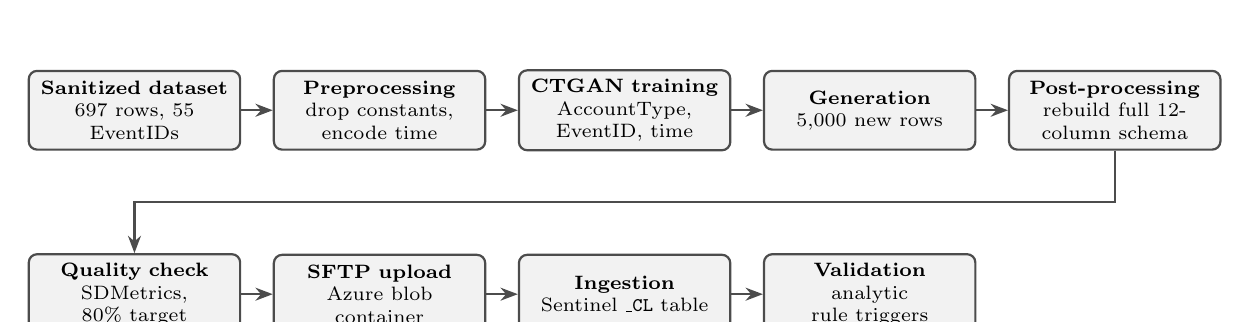
\begin{tikzpicture}[
  font=\scriptsize,
  wfbox/.style={rectangle, rounded corners=3pt, draw=black!70, fill=black!5, thick,
               text width=2.45cm, minimum height=1.0cm, align=center},
  wfpend/.style={wfbox, dashed, fill=white},
  arrow/.style={-{Stealth[length=2.2mm]}, thick, black!70}
]
% Row 1
\node[wfbox] (a1) {\textbf{Sanitized dataset}\\697 rows, 55 EventIDs};
\node[wfbox, right=0.4cm of a1] (a2) {\textbf{Preprocessing}\\drop constants, encode time};
\node[wfbox, right=0.4cm of a2] (a3) {\textbf{CTGAN training}\\AccountType, EventID, time};
\node[wfbox, right=0.4cm of a3] (a4) {\textbf{Generation}\\5,000 new rows};
\node[wfbox, right=0.4cm of a4] (a5) {\textbf{Post-processing}\\rebuild full 12-column schema};
% Row 2
\node[wfbox, below=1.3cm of a1] (b1) {\textbf{Quality check}\\SDMetrics, 80\% target};
\node[wfbox, right=0.4cm of b1] (b2) {\textbf{SFTP upload}\\Azure blob container};
\node[wfbox, right=0.4cm of b2] (b3) {\textbf{Ingestion}\\Sentinel \texttt{\_CL} table};
\node[wfbox, right=0.4cm of b3] (b4) {\textbf{Validation}\\analytic rule triggers};
% Arrows
\foreach \f/\t in {a1/a2, a2/a3, a3/a4, a4/a5, b1/b2, b2/b3, b3/b4}
  \draw[arrow] (\f) -- (\t);
\draw[arrow] (a5.south) -- ++(0,-0.65) -| (b1.north);
\end{tikzpicture}
\caption{Project Mockingbird workflow, from the sanitized dataset -> detection-rule validation.}\label{fig:workflow}
\end{figure}

% ------------------------------------------------------------
\section{Environment Setup}\label{sec:env}

\subsection{Environment overview}
\begin{itemize}
    \item Pipeline runs on an \hl{Ubuntu Desktop 26.04} virtual machine in VMware
    \item Linux was chosen because the machine learning libraries install more cleanly there than on Windows
    \item Used a virtual environment, \texttt{mockingbird-env}, to keep the projects packages separate from the system python
\end{itemize}


\subsection{Installation and dataset transfer}
The commands below set up the environment. \textbf{PyTorch} is installed in its CPU-only build because the virtual machine has no GPU. \textbf{CTGAN} is installed without its dependencies so that it does not replace that build; the missing \textbf{RDT} package is then added separately.

\begin{lstlisting}[language=bash]
# System packages
sudo apt update
sudo apt install -y python3-pip python3-venv

# Virtual environment
python3 -m venv mockingbird-env
source mockingbird-env/bin/activate

# CPU-only PyTorch (avoids multi-GB CUDA packages)
pip install torch --index-url https://download.pytorch.org/whl/cpu --no-cache-dir

# CTGAN without its default dependency pull
pip install ctgan --no-cache-dir --no-deps

# Remaining libraries
pip install sdmetrics pandas openpyxl
pip install "rdt>=1.20.0" --no-cache-dir
pip install sdv --no-cache-dir
\end{lstlisting}

\textbf{Table}~\ref{tab:libraries} lists the libraries and their roles:
\begin{table}[H]
\centering
\begin{tabular}{@{}p{3.2cm}p{9cm}@{}}
\toprule
Library & Purpose\\
\midrule
PyTorch (CPU) & Deep learning engine used by CTGAN\\
CTGAN & Generative model for tabular data\\
RDT & Encodes and decodes columns for CTGAN\\
SDMetrics & Quality score for the synthetic data\\
SDV & Metadata helper used by the evaluation script\\
pandas & Loading and transforming the datasets\\
openpyxl & Reading the \texttt{.xlsx} dataset\\
\bottomrule
\end{tabular}
\caption{Python libraries used in the project.}\label{tab:libraries}
\end{table}

\begin{itemize}
    \item The training dataset was \hl{provided internally and is already sanitized.}
\end{itemize}


\begin{figure}[H]
\centering
\includegraphics[width=0.92\textwidth]{01_env-setup_02_dataset-transferred.png}
\caption{Sanitized training dataset present on the Ubuntu virtual machine.}
\label{fig:dataset-transferred}
\end{figure}


% ------------------------------------------------------------
\section{Data Profiling}\label{sec:profiling}

\subsection{Dataset overview}
The training dataset is a sanitized sample of Windows security events in the Sentinel \texttt{SecurityEvent} format.
\begin{itemize}
    \item It has 697 rows and 12 columns
    \item 55 distinct EventIDs with about 15 rows each
    \item Profiling is done first to identify which columns the model can learn froma and which should be separated
\end{itemize}
\subsection{Profiling results}
Figure~\ref{fig:profile} shows the column types, missing values and unique-value counts.

\begin{figure}[H]
\centering
\includegraphics[height=0.65\textheight]{02_data-profiling_01_dataset-profile.png}
\caption{Dataset profile: shape, data types, null counts and unique values per column.}
\label{fig:profile}
\end{figure}

\textbf{Results:}
\begin{itemize}
  \item Five columns are constant -> so there is nothing for the model to learn.
  \item \texttt{\textbf{Account}} and \texttt{\textbf{Computer}} are unique in every row, which a GAN cannot model realistically.
  \item \texttt{\textbf{AccountType}} has 274 missing values. \texttt{\textbf{SourceSystem}} and \texttt{Level} are empty in 489 of the 697 rows, but the synthetic logs fill them on every row.
\end{itemize}

\textbf{Table}~\ref{tab:roles} gives the role of each column and how it is handled.

\begin{table}[H]
\centering
\small
\renewcommand{\arraystretch}{1.25}
\begin{tabular}{@{}>{\raggedright\arraybackslash}p{4.0cm}
                  >{\raggedright\arraybackslash}p{4.0cm}
                  >{\raggedright\arraybackslash}p{5.6cm}@{}}
\toprule
\textbf{Column} & \textbf{Role} & \textbf{Handling}\\
\midrule
\texttt{TenantId,}\newline \texttt{SourceSystem,}\newline \texttt{EventSourceName,}\newline \texttt{Channel}, \texttt{Level}
  & Constant & Set aside and reattached after generation\\
\addlinespace
\texttt{Account}, \texttt{Computer}
  & Unique in every row & Resampled from the real values\\
\addlinespace
\texttt{AccountType} & Categorical, 274 missing & Modeled: Replaced all null values with 'Unknown' so the model can learn and generate accurate output\\
\addlinespace
\texttt{EventID} & Categorical, 55 values & Modeled\\
\addlinespace
\texttt{Task} & Categorical, follows EventID & Rebuilt  from EventID\\
\addlinespace
\texttt{Activity} & Description text, one per EventID & Rebuilt from EventID\\
\addlinespace
\texttt{TimeGenerated} & Timestamp & Modeled: Converted to Unix time\\
\bottomrule
\end{tabular}
\caption{Column roles and handling.}\label{tab:roles}
\end{table}








% ------------------------------------------------------------
\section{Preprocessing}\label{sec:preprocessing}

\subsection{Purpose and steps}
\hl{Preprocessing reduces the dataset to the columns CTGAN can learn from and puts them in a form the model accepts.} The script \texttt{preprocess.py} is available in the project repository (\textcolor{blue}{\url{https://github.com/upny-hm/mockingbird/blob/main/src/preprocess.py}}).\\ It performs five steps:

\begin{enumerate}
  \item \textbf{Save the constants:} The five constant columns are stored so they can be reattached after generation.
  \item \textbf{Drop unmodeled columns:} The constants and \texttt{Activity} field are removed, since the model cannot learn from constants and \texttt{Activity} is rebuilt from \texttt{EventID} later.
  \item \textbf{Fill missing account types:} Missing \texttt{AccountType} values become ``Unknown'', which keeps every row and turns the gap into a category the model can learn.
  \item \textbf{Parse timestamps:} \texttt{TimeGenerated} is read with the ISO 8601 format, because the original timestamps have mixed fractional seconds.
  \item \textbf{Convert time to a number:} The timestamp is converted to Unix seconds, giving CTGAN a plain numeric column.
\end{enumerate}

\subsection{Implementation and output}
Figure~\ref{fig:prep-output} shows its output -> The result is saved as \texttt{preprocessed\_variable.csv}.


\begin{figure}[H]
\centering
\includegraphics[width=0.92\textwidth]{03_preprocessing_02_output.png}
\caption{Preprocessing output: constants saved and the variable columns written to CSV.}
\label{fig:prep-output}
\end{figure}
\newpage

\subsection{Verification}
A null check on the result (Figure~\ref{fig:prep-nulls}) confirms that no missing values remain.

\begin{figure}[H]
\centering
\includegraphics[width=0.92\textwidth]{03_preprocessing_03_null-check.png}
\caption{Null check on the preprocessed dataset.}
\label{fig:prep-nulls}
\end{figure}

\subsection{Issue encountered}
The first run failed while parsing \texttt{TimeGenerated}, because some timestamps have fractional seconds and others do not. Parsing with \texttt{format='ISO8601'} fixed it.

% ------------------------------------------------------------
\section{CTGAN Training}\label{sec:training}

\subsection{Model inputs}
Only the columns with learnable patterns are passed to the model (Table~\ref{tab:inputs}). \texttt{Account}, \texttt{Computer} and \texttt{Task} are excluded for the reasons given in Section~\ref{sec:profiling}.

\begin{table}[H]
\centering
\small
\renewcommand{\arraystretch}{1.25}
\begin{tabular}{@{}>{\raggedright\arraybackslash}p{4.2cm}>{\raggedright\arraybackslash}p{5cm}@{}}
\toprule
\textbf{Column} & \textbf{Type}\\
\midrule
\texttt{AccountType} & Categorical\\
\texttt{EventID} & Categorical (cast to string)\\
\texttt{TimeGenerated\_unix} & Continuous\\
\bottomrule
\end{tabular}
\caption{Columns modeled by CTGAN.}\label{tab:inputs}
\end{table}

\subsection{Configuration}


CTGAN's default batch size of 500 is almost the size of the whole 697-row dataset, so each epoch makes about one update. 
\begin{itemize}
    \item \hl{The final model was trained @ Epochs= 800 and Batch size= 50}
\end{itemize}
With a batch size of 50, 800 epochs give about 10,400 updates instead of 300, which gave the model far more chances to learn. The training script \texttt{train\_ctgan.py} is available in the project repository \textcolor{blue}{(\url{https://github.com/upny-hm/mockingbird/blob/main/src/train_ctgan.py})}, and the trained model is saved as \texttt{ctgan\_model.pkl}.

\subsection{Training runs}
The model was trained five times, changing one thing each run.The table below lists the changes and the resulting overall quality score. The scoring method is explained in \textbf{Section}~\ref{sec:quality}.

\begin{table}[H]
\centering
\small
\renewcommand{\arraystretch}{1.25}
\begin{tabular}{@{}c>{\raggedright\arraybackslash}p{6.2cm}>{\raggedright\arraybackslash}p{3cm}c@{}}
\toprule
\textbf{Run} & \textbf{Change} & \textbf{Epochs / batch} & \textbf{Score}\\
\midrule
1 & All six columns, default settings & 300 / 500 & 61.6\%\\
2 & \texttt{Account} and \texttt{Computer} removed & 300 / 500 & 68.1\%\\
3 & \texttt{Task} removed & 300 / 500 & 71.7\%\\
4 & More epochs, smaller batches & 500 / 70 & 78.4\%\\
5 & More epochs, smaller batches & 800 / 50 & 83.8\%\\
\bottomrule

\end{tabular}
\end{table}

\subsection{Final training run}
\begin{itemize}
    \item Final training run produced an overall quality score of 84\%
    \item For further information about specific training runs see: \textbf{Section}~\ref{sec:quality} 
\end{itemize}




% ------------------------------------------------------------
\section{Synthetic Data Generation}\label{sec:generation}

\subsection{Generation process}
The script \texttt{generate\_synthetic.py} is available in the project repository (\textcolor{blue}{\url{https://github.com/upny-hm/mockingbird/blob/main/src/generate_synthetic.py}}). It runs four steps:
\begin{itemize}
  \item \textbf{Sample:} load the saved model and generate 5,000 rows of \texttt{AccountType}, \texttt{EventID} and time.
  \item \textbf{Resample identities:}\hl{ fill \texttt{Account} and \texttt{Computer} with random values from the real data}, so every username and hostname is valid.
  \item \textbf{Fix types:} convert \texttt{EventID} back to an integer.
  \item \textbf{Derive Task:} look up \texttt{Task} from the generated \texttt{EventID} (Section~\ref{sec:task}).
\end{itemize}

\subsection{Deriving Task}\label{sec:task}
\begin{itemize}
  \item\textcolor{red}{\texttt{Task} is determined by \texttt{EventID}} , so it is looked up instead of generated.
  \item Some EventIDs map to more than one Task. Taking the most common one (the mode) dropped the rarer Task entirely.
  \item The final version \hl{\textbf{draws a Task at random from the values seen for that EventID in the real data, so rare Tasks keep their real frequency}.}
  \item The script prints the number of unmapped Tasks, which is 0.
\end{itemize}


\begin{figure}[H]
\centering
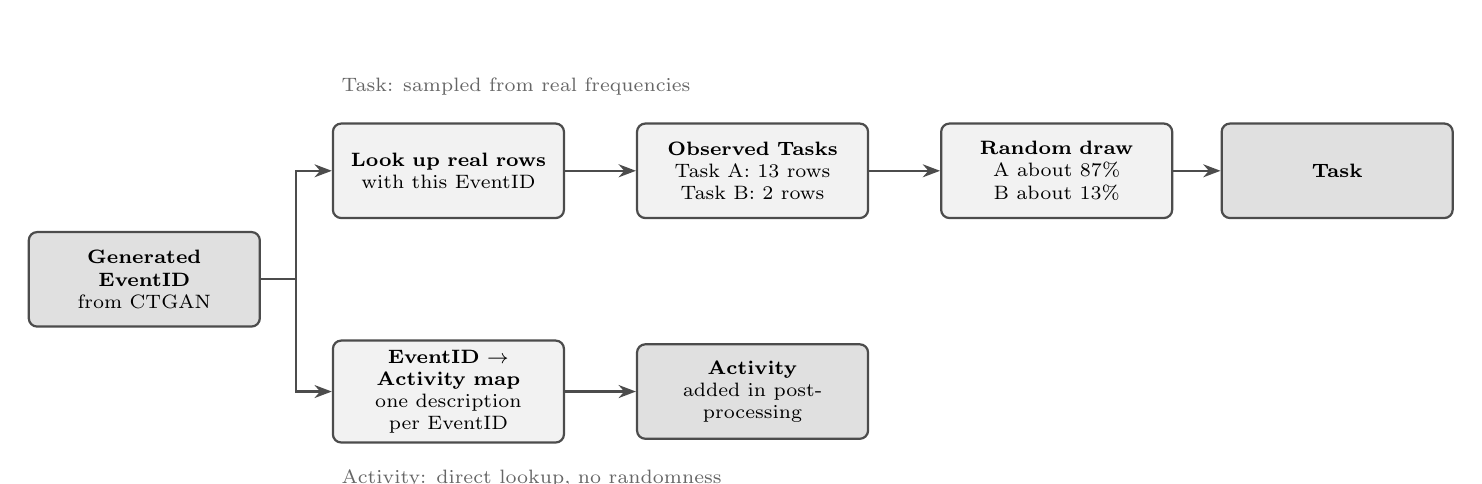
\begin{tikzpicture}[
  font=\scriptsize,
  box/.style={rectangle, rounded corners=3pt, draw=black!70, fill=black!5, thick,
              text width=2.7cm, minimum height=1.2cm, align=center},
  src/.style={box, fill=black!12},
  arrow/.style={-{Stealth[length=2.2mm]}, thick, black!70}
]
\node[src] (eid) {\textbf{Generated EventID}\\from CTGAN};

\node[box, above right=0.15cm and 0.9cm of eid] (look) {\textbf{Look up real rows}\\with this EventID};
\node[box, right=0.9cm of look] (pool) {\textbf{Observed Tasks}\\Task A: 13 rows\\Task B: 2 rows};
\node[box, right=0.9cm of pool] (draw) {\textbf{Random draw}\\A about 87\%\\B about 13\%};
\node[src, right=0.6cm of draw] (task) {\textbf{Task}};

\node[box, below right=0.15cm and 0.9cm of eid] (map) {\textbf{EventID $\to$ Activity map}\\one description per EventID};
\node[src, right=0.9cm of map] (act) {\textbf{Activity}\\added in post-processing};

\draw[arrow] (eid.east) -- ++(0.45,0) |- (look.west);
\draw[arrow] (eid.east) -- ++(0.45,0) |- (map.west);
\draw[arrow] (look) -- (pool);
\draw[arrow] (pool) -- (draw);
\draw[arrow] (draw) -- (task);
\draw[arrow] (map) -- (act);

\node[anchor=west, text=black!60] at ($(look.north west)+(0,0.45)$) {Task: sampled from real frequencies};
\node[anchor=west, text=black!60] at ($(map.south west)+(0,-0.45)$) {Activity: direct lookup, no randomness};
\end{tikzpicture}
\caption{How \texttt{Task} and \texttt{Activity} are derived from the generated \texttt{EventID}.}
\label{fig:derive}
\end{figure}



\subsection{Script versions and output}
\begin{itemize}
  \item \textbf{First version:} samples all rows straight from the model (Figure~\ref{fig:gen-v1}). The output has the expected six fields (Figure~\ref{fig:gen-fields}).
  \item \textbf{Validity check:} every categorical value in the synthetic data also exists in the real data, with 0 unseen values (Figure~\ref{fig:gen-check}).
  \item \textbf{Second version:} \texttt{Account} and \texttt{Computer} are resampled from the real pool (Figure~\ref{fig:gen-v2}). The run produces 5,000 rows with 6 columns (Figure~\ref{fig:gen-run}).
  \item \textbf{Final version:} adds the probabilistic Task lookup (Figure~\ref{fig:gen-final}).
\end{itemize}



\begin{figure}[H]
\centering
\includegraphics[width=0.92\textwidth]{05_synthetic-generation_01_script.png}
\caption{First version of the generation script.}
\label{fig:gen-v1}
\end{figure}

\begin{figure}[H]
\centering
\includegraphics[width=0.92\textwidth]{05_synthetic-generation_02_output.png}
\caption{Synthetic data fields and sample rows from the first version.}
\label{fig:gen-fields}
\end{figure}

\begin{figure}[H]
\centering
\includegraphics[width=0.92\textwidth]{05_synthetic-generation_03_format-validation.png}
\caption{Check for synthetic values that do not exist in the real data.}
\label{fig:gen-check}
\end{figure}

\begin{figure}[H]
\centering
\includegraphics[width=0.92\textwidth]{05_synthetic-generation_04_updated-script.png}
\caption{Second version: \texttt{Account} and \texttt{Computer} resampled from the real pool.}
\label{fig:gen-v2}
\end{figure}

\begin{figure}[H]
\centering
\includegraphics[width=0.92\textwidth]{05_synthetic-generation_05_updated-output.png}
\caption{Run of the second version: 5,000 rows, 6 columns.}
\label{fig:gen-run}
\end{figure}

\begin{figure}[H]
\centering
\includegraphics[width=0.92\textwidth]{05_synthetic-generation_07_probabilistic-task-script.png}
\caption{Final script with probabilistic Task derivation.}
\label{fig:gen-final}
\end{figure}





% ------------------------------------------------------------
\section{Post-processing}\label{sec:postprocessing}

\subsection{Purpose and steps}
The model output has only six columns, while Sentinel expects the full 12-column {\texttt{SecurityEvent}} schema. The script \texttt{postprocess.py} (\url{https://github.com/upny-hm/mockingbird/blob/main/src/postprocess.py}) rebuilds it in five steps:
\begin{itemize}
  \item \textbf{Build the lookup:} map each \texttt{EventID} \textbf{->} \texttt{Activity} using the original dataset.
  \item \textbf{Add Activity:} fill \texttt{Activity} on every row, with 0 unmapped.
  \item \textbf{Reattach constants:} restore \texttt{TenantId}, \texttt{SourceSystem}, \texttt{EventSourceName}, \texttt{Channel} and \texttt{Level}.
  \item \textbf{Restore timestamps:} convert Unix time back to the Sentinel format \\ \texttt{YYYY-MM-DDTHH:mm:ss.fffZ}.
  \item \textbf{Reorder columns:} match the original schema and save \texttt{synthetic\_final.csv}.
\end{itemize}
\texttt{Activity} is copied exactly as it appears in the original data, so a few EventIDs keep their original placeholder text (such as ``-'').

\subsection{Output}
\begin{itemize}
  \item The result is 5,000 rows by 12 columns (about 1 MB).
  \item Figure~\ref{fig:post-script} shows the script, Figure~\ref{fig:post-run} shows the run, and Figure~\ref{fig:post-sample} shows a sample of the final file.
\end{itemize}

\begin{figure}[H]
\centering
\includegraphics[width=0.92\textwidth]{06_post-processing_01_script.png}
\caption{The post-processing script.}
\label{fig:post-script}
\end{figure}

\begin{figure}[H]
\centering
\includegraphics[width=0.92\textwidth]{06_post-processing_02_output.png}
\caption{Post-processing run: 12 columns, 5,000 rows, 0 unmapped Activity.}
\label{fig:post-run}
\end{figure}

\begin{figure}[H]
\centering
\includegraphics[width=0.92\textwidth]{06_post-processing_05_final-sample.png}
\caption{Sample rows from \texttt{synthetic\_final.csv}.}
\label{fig:post-sample}
\end{figure}

\subsection{Format validation}
\begin{itemize}
  \item A regular-expression check on \texttt{synthetic\_final.csv} tests the three formats named in the success criteria: IP addresses (\texttt{Computer}), usernames (\texttt{Account}) and timestamps (\texttt{TimeGenerated}).
  \item The check is implemented through the script \texttt{validate\_format.py} (\url{https://github.com/upny-hm/mockingbird/blob/main/src/validate_format.py}).
  \item It reports the share of rows matching each pattern, for both the original and the synthetic data. The target is 100\%.
\end{itemize}

\begin{figure}[H]
\centering
\includegraphics[width=0.92\textwidth]{06_post-processing_06_format-validation.png}
\caption{Format validation of IP addresses, usernames and timestamps.}
\label{fig:post-format}
\end{figure}








% ------------------------------------------------------------
\section{Quality Evaluation}\label{sec:quality}

\subsection{Method}
\begin{itemize}
  \item The SDMetrics \texttt{QualityReport} compares the synthetic data with the real data. The script \texttt{evaluate\_quality.py} is available in the project repository (\textcolor{blue}{\url{https://github.com/upny-hm/mockingbird/blob/main/src/evaluate_quality.py}}).
  \item \textbf{Column Shapes:} does each column's distribution match the real one?
  \item \textbf{Column Pair Trends:} do the relationships between pairs of columns match?
  \item \textbf{Overall score:} the average of the two -> The target is 80\%.
  \item \textbf{NOTE:} The final version scores only the modeled columns (\texttt{AccountType}, \texttt{EventID} and time), because the other columns are either resampled or derived.
\end{itemize}

\subsection{Tuning progression}
\begin{itemize}
  \item The model was tuned over five runs (Table 4). Figure~\ref{fig:progress} summarizes the scores, and Figures~\ref{fig:q-script1} to~\ref{fig:q-run5} show the evidence for each run.
  \item Runs 2 and 3 score fewer columns than run 1, so only runs 3 to 5 are directly comparable.
\end{itemize}

\begin{figure}[H]
\centering
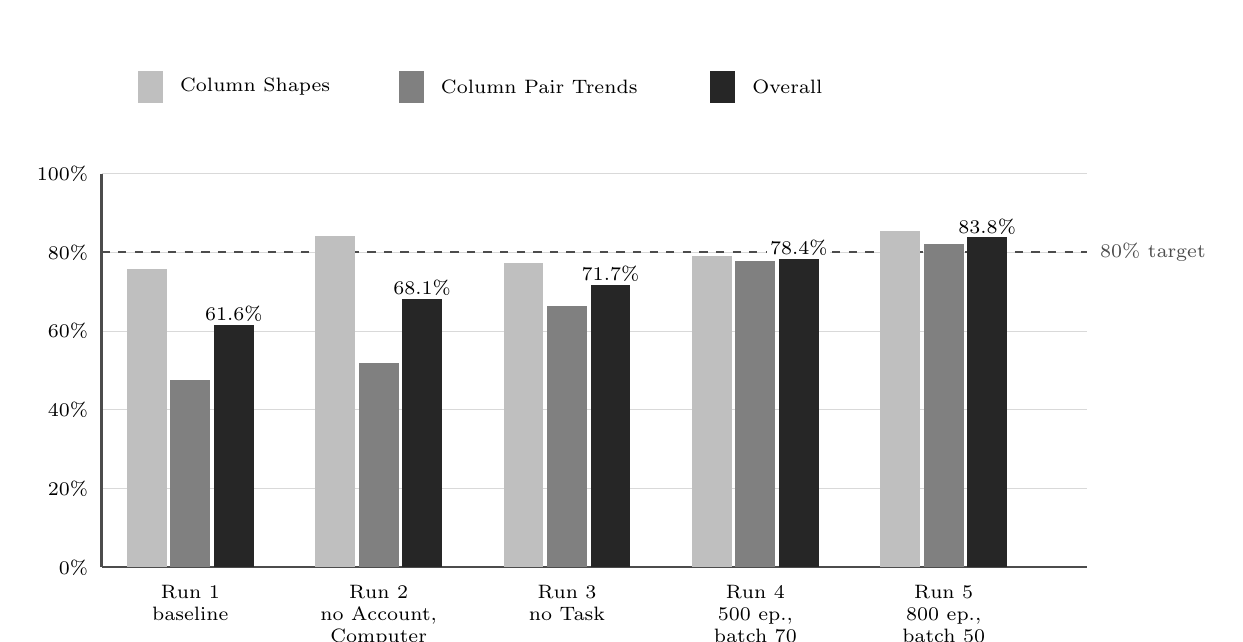
\begin{tikzpicture}[font=\scriptsize, x=0.92cm, y=0.05cm]
  \foreach \v in {0,20,40,60,80,100} {
    \draw[black!15] (-0.5,\v) -- (13.1,\v);
    \node[anchor=east] at (-0.55,\v) {\v\%};
  }
  \draw[thick, black!70] (-0.5,0) -- (13.1,0);
  \draw[thick, black!70] (-0.5,0) -- (-0.5,100);
  \draw[dashed, thick, black!70] (-0.5,80) -- (13.1,80);
  \node[anchor=west, text=black!70] at (13.15,80) {80\% target};
  \foreach \i/\s/\t/\o/\lab in {
    0/75.7/47.6/61.6/{Run 1\\baseline},
    1/84.2/51.9/68.1/{Run 2\\no Account,\\Computer},
    2/77.2/66.3/71.7/{Run 3\\no Task},
    3/79.1/77.7/78.4/{Run 4\\500 ep.,\\batch 70},
    4/85.5/82.2/83.8/{Run 5\\800 ep.,\\batch 50}} {
    \pgfmathsetmacro{\x}{\i*2.6+0.7}
    \fill[black!25] (\x-0.85,0) rectangle (\x-0.3,\s);
    \fill[black!50] (\x-0.25,0) rectangle (\x+0.3,\t);
    \fill[black!85] (\x+0.35,0) rectangle (\x+0.9,\o);
    \node[above, fill=white, inner sep=1pt] at (\x+0.625,\o) {\o\%};
    \node[below, align=center] at (\x+0.025,-2) {\lab};
  }
  \fill[black!25] (0,118) rectangle (0.35,126); \node[anchor=west] at (0.45,122) {Column Shapes};
  \fill[black!50] (3.6,118) rectangle (3.95,126); \node[anchor=west] at (4.05,122) {Column Pair Trends};
  \fill[black!85] (7.9,118) rectangle (8.25,126); \node[anchor=west] at (8.35,122) {Overall};
\end{tikzpicture}
\caption{Quality score progression across the five training runs.}
\label{fig:progress}
\end{figure}

\begin{figure}[H]
\centering
\includegraphics[width=0.92\textwidth]{07_sdmetrics_00_script.png}
\caption{Run 1 script: baseline evaluation of all six columns with default training settings.}
\label{fig:q-script1}
\end{figure}

\begin{figure}[H]
\centering
\includegraphics[width=0.92\textwidth]{07_sdmetrics_01_initial-score.png}
\caption{Run 1 result: overall 61.6\% (shapes 75.7\%, pair trends 47.6\%).}
\label{fig:q-run1}
\end{figure}

\begin{figure}[H]
\centering
\includegraphics[width=0.92\textwidth]{07_sdmetrics_03_updated-script.png}
\caption{\texttt{Account} and \texttt{Computer} are unique in all 697 rows, so the model cannot learn them -> Both fields were removed.}
\label{fig:q-unique}
\end{figure}

\begin{figure}[H]
\centering
\includegraphics[width=0.92\textwidth]{07_sdmetrics_04_updated-score.png}
\caption{Run 2 script: \texttt{Account} and \texttt{Computer} removed from the model and the evaluation [Score = 68\%].}
\label{fig:q-script2}
\end{figure}

\begin{figure}[H]
\centering
\includegraphics[width=0.92\textwidth]{07_sdmetrics_05_final-script.png}
\caption{Script was updated to also remove \texttt{task} from the evaluation since it is derived from \texttt{EventID} not generated by the model.}
\label{fig:q-run2}
\end{figure}

\begin{figure}[H]
\centering
\includegraphics[width=0.92\textwidth]{07_sdmetrics_06_score-71pct.png}
\caption{Run 3 script: \texttt{Task}  removed, overall score increased 72\%}
\label{fig:q-script3}
\end{figure}


\begin{figure}[H]
\centering
\includegraphics[width=0.92\textwidth]{07_sdmetrics_08_score-84pct.png}
\caption{Run 4 result: overall 78.4\% (shapes 79.1\%, pair trends 77.7\%) after retraining with 500 epochs and batch size 70.}
\label{fig:q-run4}
\end{figure}

\begin{figure}[H]
\centering
\includegraphics[width=0.92\textwidth]{07_sdmetrics_08_score-84pct.png}
\caption{Run 5 result: overall 83.8\% (shapes 85.5\%, pair trends 82.2\%) after retraining with 800 epochs and batch size 50.}
\label{fig:q-run5}
\end{figure}

\subsection{Final result}
\begin{itemize}
  \item The final model scored 83.8\%, above the 80\% target, so the Data fidelity criteria is met.
\end{itemize}










% ------------------------------------------------------------
\section{Sentinel Integration}\label{sec:integration}

\subsection{Overview}
\begin{itemize}
  \item This stage pushed \texttt{synthetic\_final.csv} from the virtual machine into a Microsoft Sentinel custom log table.
  \item The file is stored in an Azure Blob container over SFTP, and the records are pushed to the \texttt{GAN\_CL\_CL} table through the Azure Monitor Logs Ingestion API (Figure~\ref{fig:integration}).
\end{itemize}

\begin{figure}[H]
\centering
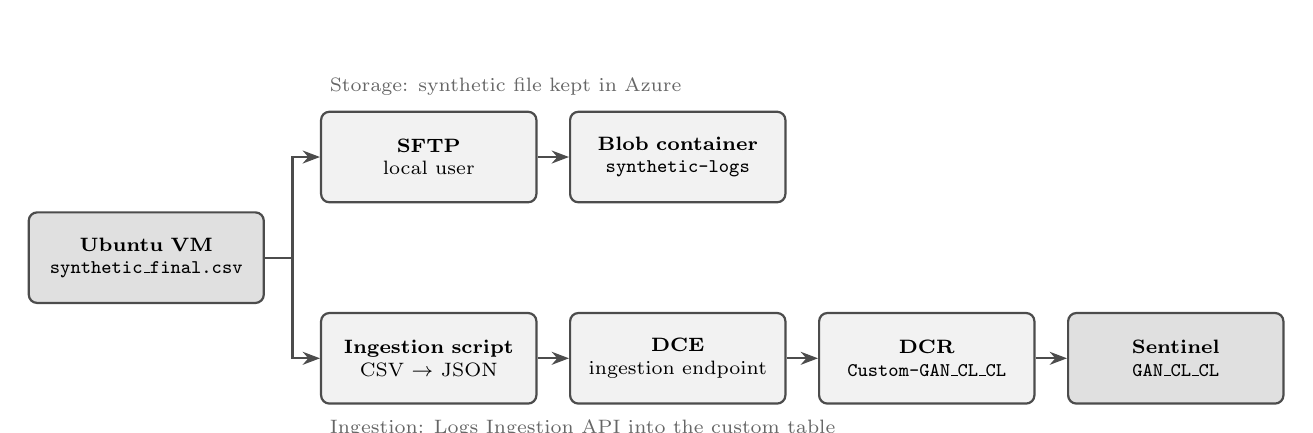
\begin{tikzpicture}[
  font=\scriptsize,
  box/.style={rectangle, rounded corners=3pt, draw=black!70, fill=black!5, thick,
              text width=2.5cm, minimum height=1.15cm, align=center},
  src/.style={box, fill=black!12},
  arrow/.style={-{Stealth[length=2.2mm]}, thick, black!70}
]
\node[src, text width=2.75cm] (vm) {\textbf{Ubuntu VM}\\\texttt{synthetic\_final.csv}};
\node[box, above right=0.1cm and 0.7cm of vm] (sftp) {\textbf{SFTP}\\local user};
\node[box, right=0.4cm of sftp] (blob) {\textbf{Blob container}\\\texttt{synthetic-logs}};
\node[box, below right=0.1cm and 0.7cm of vm] (script) {\textbf{Ingestion script}\\CSV $\to$ JSON};
\node[box, right=0.4cm of script] (dce) {\textbf{DCE}\\ingestion endpoint};
\node[box, right=0.4cm of dce] (dcr) {\textbf{DCR}\\\texttt{Custom-GAN\_CL\_CL}};
\node[src, right=0.4cm of dcr] (tbl) {\textbf{Sentinel}\\\texttt{GAN\_CL\_CL}};
\draw[arrow] (vm.east) -- ++(0.35,0) |- (sftp.west);
\draw[arrow] (vm.east) -- ++(0.35,0) |- (script.west);
\draw[arrow] (sftp) -- (blob);
\draw[arrow] (script) -- (dce);
\draw[arrow] (dce) -- (dcr);
\draw[arrow] (dcr) -- (tbl);
\node[anchor=west, text=black!60] at ($(sftp.north west)+(0,0.3)$) {Storage: synthetic file kept in Azure};
\node[anchor=west, text=black!60] at ($(script.south west)+(0,-0.3)$) {Ingestion: Logs Ingestion API into the custom table};
\end{tikzpicture}
\caption{Integration architecture.}
\label{fig:integration}
\end{figure}

\subsection{Storage account and SFTP upload}
\begin{itemize}
  \item \textbf{Storage account:} \texttt{ctgandataset}, with hierarchical namespace and SFTP enabled.
  \item \textbf{Container:} \texttt{synthetic-logs} holds the synthetic dataset.
  \item \textbf{Access:} a local SFTP user authenticated with an SSH password.
  \item \textbf{Upload:} the file was uploaded over SFTP from the Windows host, because the virtual machine had no network access at the time.
\end{itemize}

\begin{figure}[H]
\centering
\includegraphics[width=0.92\textwidth]{08_sentinel-ingestion_01_storage-account-created.png}
\caption{Storage account \texttt{ctgandataset}.}
\label{fig:storage-account}
\end{figure}

\begin{figure}[H]
\centering
\includegraphics[width=0.92\textwidth]{08_sentinel-ingestion_02_hierarchical-namespace-enabled.png}
\caption{Hierarchical namespace and SFTP enabled on the storage account.}
\label{fig:storage-hns}
\end{figure}

\begin{figure}[H]
\centering
\includegraphics[width=0.92\textwidth]{08_sentinel-ingestion_03_container-created.png}
\caption{Blob container \texttt{synthetic-logs}.}
\label{fig:storage-container}
\end{figure}

\begin{figure}[H]
\centering
\includegraphics[width=0.92\textwidth]{08_sentinel-ingestion_04_local-user-created.png}
\caption{Local SFTP user created for the upload.}
\label{fig:storage-user}
\end{figure}

\begin{figure}[H]
\centering
\includegraphics[width=0.92\textwidth]{08_sentinel-ingestion_06_file-uploaded.png}
\caption{\texttt{synthetic\_final.csv} uploaded to the container over SFTP.}
\label{fig:storage-upload}
\end{figure}

\subsection{Custom table and data collection rule}
\begin{itemize}
  \item \textbf{Custom table:} \texttt{GAN\_CL\_CL} in the Log Analytics workspace receives the synthetic records.
  \item \textbf{Data collection endpoint (DCE):} the URL the records are sent to.
  \item \textbf{Data collection rule (DCR):} declares the input stream \texttt{Custom-GAN\_CL\_CL}, its columns and types, and routes the records into the table.
  \item \textbf{Permission:} the \textit{Monitoring Metrics Publisher} role on the DCR allows the ingestion script to send data.
\end{itemize}

\begin{figure}[H]
\centering
\includegraphics[width=0.92\textwidth]{08_sentinel-ingestion_08_custom-table.png}
\caption{DCR JSON view: input stream \texttt{Custom-GAN\_CL\_CL} and its columns.}
\label{fig:dcr-json}
\end{figure}



\begin{figure}[H]
\centering
\includegraphics[width=0.92\textwidth]{08_sentinel-ingestion_09_dcr-role.png}
\caption{Monitoring Metrics Publisher role assigned on the DCR.}
\label{fig:dcr-role}
\end{figure}

\subsection{Ingestion script}
The script \texttt{ingest\_to\_sentinel.py} is available in the project repository (\textcolor{blue}{\url{https://github.com/upny-hm/mockingbird/blob/main/src/ingest_to_sentinel.py}}). It runs these steps:
\begin{itemize}
  \item \textbf{Read:} load \texttt{synthetic\_final.csv}. The final upload used the local copy on the virtual machine.
  \item \textbf{Drop \texttt{TenantId}:} it is a reserved column name in Log Analytics, which fills it automatically.
  \item \textbf{Set types:} \texttt{Task} and \texttt{EventID} as integers, all other columns as text.
  \item \textbf{Shift timestamps:} map the original time range into the last 24 hours, keeping order and spacing. Azure replaces timestamps older than two days, and analytic rules only search recent data.
  \item \textbf{Convert:} turn each row into a JSON record.
  \item \textbf{Authenticate:} sign in with a device code.
  \item \textbf{Upload:} send the records to the DCE and DCR. The Azure SDK splits them into chunks under the 1~MB request limit.
\end{itemize}

\begin{figure}[H]
\centering
\includegraphics[width=0.92\textwidth]{08_sentinel-ingestion_10_full-upload.png}
\caption{Ingestion run: 5,000 records sent, 0 failed.}
\label{fig:full-upload}
\end{figure}

\subsection{Verification}
\begin{itemize}
  \item A query on \texttt{GAN\_CL\_CL} counts the records and checks that every column is populated (Figure~\ref{fig:records-in-table}).
  \item The table holds 5,009 records: the 5,000 synthetic rows plus 10 rows from an initial test upload, which remain in the table.
  \item Every column is filled in every row, so the data was ingested without parsing errors and the Integration criterion is met.
\end{itemize}

\begin{figure}[H]
\centering
\includegraphics[width=0.92\textwidth]{08_sentinel-ingestion_11_records-in-table.png}
\caption{Records in \texttt{GAN\_CL\_CL} with all columns populated.}
\label{fig:records-in-table}
\end{figure}





% ------------------------------------------------------------
\section{Validation}\label{sec:validation}

\subsection{Approach}
\begin{itemize}
  \item Organizational analytic rules and incidents are \textcolor{red}{confidential} and are not reproduced in this report. Instead validation was carried out at he Query level: a password spray detection query was run against \texttt{GAN\_CL\_CL} in the Sentinel workspace.
  \item Every event the query evaluates was generated by CTGAN. No attack events were added by hand.
\end{itemize}

\subsection{Password spray detection}
A password spray tries one or two common passwords against many accounts, so it shows up as many accounts failing to log on within a short time. The query looks for three signs of this, in one-hour windows:
\begin{itemize}
  \item \textbf{High volume of failed logons:} \texttt{FailedAttempts}, and \texttt{SpikeRatio} against the normal hourly rate (the median over the last day = 2 failed attmpts per account).
  \item \textbf{Failed logons against active users:} \texttt{ActiveTargeted}, the accounts that also logged on successfully in the same period.
  \item \textbf{Failed logons for nonexistent accounts:} \texttt{UnknownTargeted}, accounts that never appear outside failed logons.
\end{itemize}
A window is flagged when at least 20 accounts fail and failures are at least 10 times the normal rate. Severity is High if nonexistent accounts are targeted or failures are at least 50 times the normal rate, and Medium otherwise.


\begin{figure}[H]
\centering
\includegraphics[width=0.92\textwidth]{09_validation_01_spray-query.png}
\caption{Password spray detection query in the Sentinel Logs editor.}
\label{fig:spray-query}
\end{figure}

\subsection{Results}
The query returned two detections (Figure~\ref{fig:spray-output}). The full output is available in the project repository. (\textcolor{blue}{\url{https://github.com/upny-hm/mockingbird/blob/main/src/data/KQL_query_output.csv}})

\begin{figure}[H]
\centering
\includegraphics[width=1\textwidth]{09_validation_02_query-ouput.png}
\caption{Query output: two flagged one-hour windows.}
\label{fig:spray-output}
\end{figure}

\begin{itemize}
  \item \textbf{One attempt, two time windows:} the two detections are back to back. \\ \textbf{6:23:16 AM - 6:59:14 AM} recorded 143 failed login attempts and a 61.6 spike ratio which set off the rule. \textbf{7:00:06 AM - 7:22:39 AM} also saw 43 failed login attempts and a spike ration of 21.6 Spike Ratio which also set off the rule.
  \item \textbf{Distributed pattern:} failures came from more than 100 different source IPs, indicating a password spray attempt, where attempts are spread across many sources to stay below normal failed login thresholds.
  \item \textbf{Active users targeted:} 29 and 10 of the targeted accounts had logged on successfully in the same period.
  \item \textbf{No nonexistent accounts:} \texttt{UnknownTargeted} is 0, because CTGAN can only reuse account names it saw during training.
  \item \textbf{Cause of the burst:} most events fall into a short period, because CTGAN reproduced the busy period of the original data and the timestamps were mapped into the last 24 hours. The share of failed logons inside the burst is the same as across the whole dataset, so the detection reflects a surge in volume rather than an attack-specific pattern.
\end{itemize}


\begin{figure}
    \centering
    \includegraphics[width=1\linewidth]{KQL_flow.png}
    \caption{KQl query logic}
    \label{fig:placeholder}
\end{figure}





% ------------------------------------------------------------
\section{Conclusion}\label{sec:conclusion}

Project Mockingbird showed that a CTGAN model trained on a small, sanitized sample of Windows security events can generate realistic synthetic logs, deliver them into Microsoft Sentinel, and trigger detection logic, without exposing real user data. All four success criteria were met:

\begin{itemize}
  \item \textbf{Data fidelity:} the final model scored 83.8\% on the SDMetrics quality report, above the 80\% target (Section~\ref{sec:quality}).
  \item \textbf{Formatting:} IP addresses, usernames and timestamps in the synthetic data matched the original formats (Section~\ref{sec:postprocessing}).
  \item \textbf{Integration:} 5,000 synthetic records were ingested into the \texttt{GAN\_CL\_CL} custom table with every column populated (Section~\ref{sec:integration}).
  \item \textbf{Validation:} a password spray detection query flagged the CTGAN-generated data in Sentinel (Section~\ref{sec:validation}).
\end{itemize}

The project also showed the limits of a row-based generator. CTGAN learns what individual events look like, but not patterns that span many events, so it cannot produce targeted attack sequences or invent new account names on its own. Training on labeled attack examples, or using a generator that models event sequences, would let future work produce specific attack scenarios on demand. Even in its current form, the pipeline gives the SOC a repeatable, \hl{privacy-safe way to generate test data and check detection logic}.

\end{document}
